%%%%%%%%%%%%%%%%%%%%%%%%%%%%%%%%%%%%%%%%%%%%%%%%%%%%%%%%%%%%%%%%%%%%%
% LaTeX Template: Project Titlepage Modified (v 0.1) by rcx
%
% Original Source: http://www.howtotex.com
% Date: February 2014
% 
% This is a title page template which be used for articles & reports.
% 
% This is the modified version of the original Latex template from
% aforementioned website.
% 
%%%%%%%%%%%%%%%%%%%%%%%%%%%%%%%%%%%%%%%%%%%%%%%%%%%%%%%%%%%%%%%%%%%%%%

\documentclass[10pt]{report}
\usepackage{booktabs}
\usepackage[a4paper]{geometry}
\usepackage[myheadings]{fullpage}
\usepackage{fancyhdr}
\usepackage{lastpage}
\usepackage{mathtools}
\usepackage{float}
\DeclarePairedDelimiter\ceil{\lceil}{\rceil}
\DeclarePairedDelimiter\floor{\lfloor}{\rfloor}
\usepackage{multirow}
\usepackage{breakcites}
\usepackage{graphics}
\usepackage{graphicx, wrapfig, subcaption, setspace, booktabs}
\usepackage[T1]{fontenc}
\usepackage[font=small, labelfont=bf]{caption}
\usepackage{fourier}
\usepackage[protrusion=true, expansion=true]{microtype}
\usepackage[english]{babel}
\usepackage{sectsty}
\usepackage{lscape}
\usepackage{url, lipsum}
\usepackage[hidelinks]{hyperref}
\usepackage{xcolor}
\renewcommand{\thesection}{\arabic{section}}
\newcommand{\HRule}[1]{\rule{\linewidth}{#1}}
\onehalfspacing

\begin{document}
{\fontfamily{cmr}\selectfont
\title{ \normalsize \textsc{}
		\\ [2.0cm]
		\HRule{0.5pt} \\
		 \textbf{\uppercase{Analysis Report} \\
		\LARGE Intelligent test interface with Plagiarism Detection\\
		\Large {(Software Lab Course Project)}
		\HRule{2pt} \\ [0.5cm]
		\normalsize \today \vspace*{5\baselineskip}}
		}
\date{}
\author{
  Jay Bansal\\
  \texttt{193050004}
  \and
  Sriniwas Paliwal\\
  \texttt{193050042} \\ \\
  (TEAM INFERNOS)
  \and
  Harmeen Kaur\\
  \texttt{193050020} 
}
\maketitle
\tableofcontents
%-------------------------------------------------------------------------------
% Section title formatting


%-------------------------------------------------------------------------------

%-------------------------------------------------------------------------------
% BODY
%-------------------------------------------------------------------------------
\begin{abstract}
This project work develops an intelligent test interface which helps detecting the plagiarism among responses submitted by various students. Test can be created by admin and floated among students. Test taker can choose to apply plagiarism test, also he can constraint which algorithm to apply for plagiarism index evaluation. This work also includes analysis of various string matching algorithms and python libraries implementing different string similarity and distance measures. Ultimately discovered algorithm will provide weights to different algorithms to come up with the best accurate plagiarism index between students.
This model can help mitigating the inconsistencies which arise while detecting plagiarism manually in traditional manner, also this can be a lengthy and time-consuming task for the reader but Plagiarism detection model we built will evaluate it automatically in no time.
\end{abstract}
\section{Introduction}
\subsection{Motivation}

Plagiarism is the practice of taking credit for someone else's words or ideas. It's an act of intellectual dishonesty. In colleges and universities, it violates honor codes. Presenting others' work without adequate acknowledgement of its source, as though it were one’s own is
Plagiarism and it is clearly a form of fraud. \\
Some forms of plagiarism are obvious. Copying someone else's essay word for word and submitting it as your own but more complex forms of plagiarism exist which might be difficult to capture by simple algorithms. \\
Some forms of Plagiarism are :
\begin{enumerate}
    \item \textbf{Direct plagiarism} is the act of copying another person's work word for word. Inserting a paragraph from a book or article into your essay without including attribution.
    \item \textbf{Paraphrased plagiarism} involves making a few (often cosmetic) changes to someone else’s work, then passing it off as your own.
    \item \textbf{Mosaic plagiarism} is a combination of direct and paraphrased plagiarism. This type involves tossing various words, phrases, and sentences (some word for word, some paraphrased) into your essay without providing attributions.
    \item \textbf{Accidental plagiarism} occurs when citations are missing, sources are cited incorrectly, or an author shares an idea without a citation that isn't as common of knowledge as they thought. Accidental plagiarism is often the result of a disorganized research process and a last-minute time crunch. \cite{plag}
\end{enumerate}
Plagiarism detection is the process of locating instances of plagiarism within a work or document. \cite{wiki}Detection of plagiarism can be undertaken in a variety of ways. Human detection is the most traditional form of identifying plagiarism from written work. This can be a lengthy and time-consuming task for the reader and can also result in inconsistencies in how plagiarism is identified within an organization. So the better way is to use automatically plagiarism detectors to save time and efforts.  

\subsection{Objective}
Goal is to build an efficient algorithm which performs optimal plagiarism detection task on the given set of test responses and provide us with a fair index of plagiarism corresponding to each response. And to build an interface which let Test taker to set tests and student to access the live tests and submit responses.



\section{Approach to the problem}
The test may have various type of questions:
\begin{enumerate}
    \item Multiple Choice Questions Choose Single Answer
    \item Multiple Choice Questions Choose Multiple Answers
    \item Subjective Answer Single Line
    \item Subjective Answer Multiple lines
\end{enumerate}

Starting with the subjective answers, we need to apply string matching algorithms in such a way that it gives optimal metric index of match.For this purpose, we explored \textbf{strsim}, A library implementing different string similarity and distance measures. It currently includes a dozen of string matching algorithms implemented.\cite{strsim} Some of those which we found beneficial for the task supposed be done, are as following:
\begin{itemize}
    \item \textbf{Longest Common Subsequence :} LCS gives the size of the longest subsequence which is common to both the given strings.
    The LCS distance between strings X (of length n) and Y (of length m) is \\  n + m - 2 |LCS(X, Y)| min = 0 max = n + m
    \item \textbf{Normalized Levenshtein :}The Levenshtein distance between two words is the minimum number of single-character edits (insertions, deletions or substitutions) required to change one word into the other.
    The levenshtein distance divided by the length of the longest string results in a value that is always in the interval [0.0 1.0]. This is Normalized Levenshtein distance.The similarity is computed as 1 - normalized distance.
    
    \item \textbf{Metric Longest Common Subsequence :} It is a measure of distance metric based on Longest Common Subsequence explained earlier. It is computed as: \\
    \begin{equation}
     1 - |LCS(s1, s2)| / max(|s1|, |s2|)
     \end{equation}
    \item \textbf{Shingle (N-gram) based algorithms :}An n-gram is a contiguous sequence of n items from a given sample of text or speech. The items can be phonemes, syllables, letters, words or base pairs according to the application. The n-grams typically are collected from a text or speech corpus. When the items are words, n-grams may also be called shingles. An n-gram of size 1 is referred to as a unigram, size 2 is a bigram and size 3 is a trigram. These are effectively used in string matching algorithms.\\ 
    A few algorithms work by converting strings into sets of n-grams (sequences of n characters, also sometimes called k-shingles). The similarity or distance between the strings is then the similarity or distance between the sets.
    \\ Some of n-gram based algorithms are as follows: 
    \begin{itemize}
        \item \textbf{Q-Gram : }The distance between two strings is defined as the L1 norm of the difference of their profiles (the number of occurences of each n-gram): SUM( $|V1_i - V2_i|$ ). Q-gram distance is a lower bound on Levenshtein distance, but can be computed in O(m + n), where Levenshtein requires O(m.n)
        \item \textbf{Cosine similarity: }The similarity between the two strings is the cosine of the angle between these two vectors representation, and is computed as: \\
        \begin{equation}
        V1 . V2 / (|V1| * |V2|) 
        \end{equation}
        Distance is computed as 1 - cosine similarity.

        \item \textbf{Jaccard index : }Like Q-Gram distance, the input strings are first converted into sets of n-grams (sequences of n characters, also called k-shingles), but this time the cardinality of each n-gram is not taken into account. Each input string is simply a set of n-grams. The Jaccard index is then computed as: \\ 
        \begin{equation}
        |V1 \cap V2| / |V1 \cup V2|
        \end{equation}
    \end{itemize}
\item \textbf{Cosine\_similarity\_word : } This is a modified version of cosine angle similarity measure. There we compare two strings' similarity by making two vectors having entries of frequency of distinct letters in it. Here we are picking word by word and vectors are formed on frequency of words. IT works very effectively, That's why we will be high weight to this algorithm as well.
\end{itemize}

\section{Layout and Flow of Project}
\subsection{Front End}
We are using wordpress \cite{word} for front end design. We created a website on which it displays all the live tests student can attempt and submit. We are using Ninja plugin in wordpress for creating tests online and publishing the same. The test must have a roll number field which will be used to identify the student. For now any student visiting the website can attempt any of the displayed live tests. About setting the test, Admin is the only teacher yet which can set test and publish it online on website. \\
\begin{figure}[H]
    \centering
    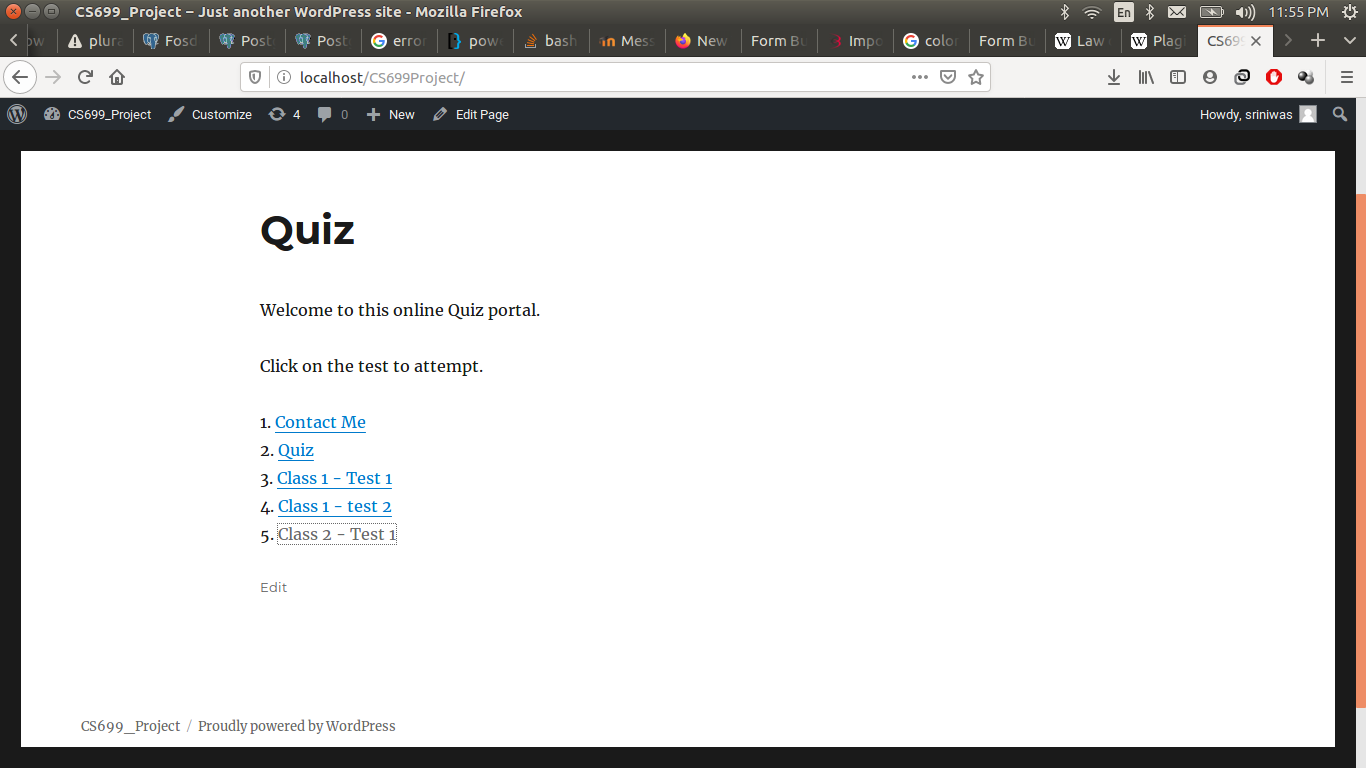
\includegraphics[width=0.5\paperwidth]{images/Website.png}
    \caption{A small overlook of the website}
    \label{fig:galaxy}
\end{figure}

Here are some tests we have already published for testing and analysis purpose. Students can attempt to submit responses for these tests. The asterisk mark fields are mandatory to fill, otherwise form will not get submitted.
\begin{figure}[H]
\label{fig1}
      \centering
  \begin{minipage}[b]{0.45\textwidth}
    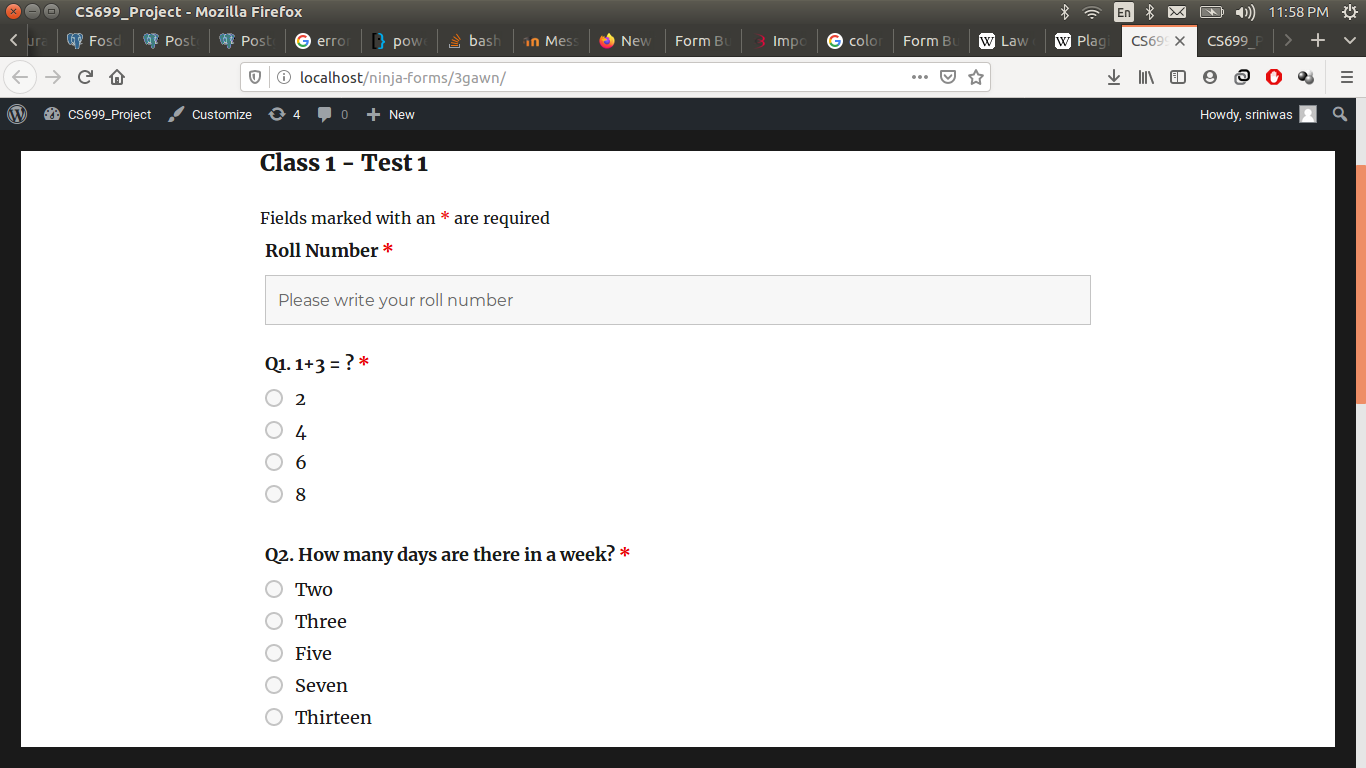
\includegraphics[width=\textwidth]{images/Test11.png}
    \caption{Demo Test1 Page 1}
  \end{minipage}
  \hfill
  \begin{minipage}[b]{0.45\textwidth}
    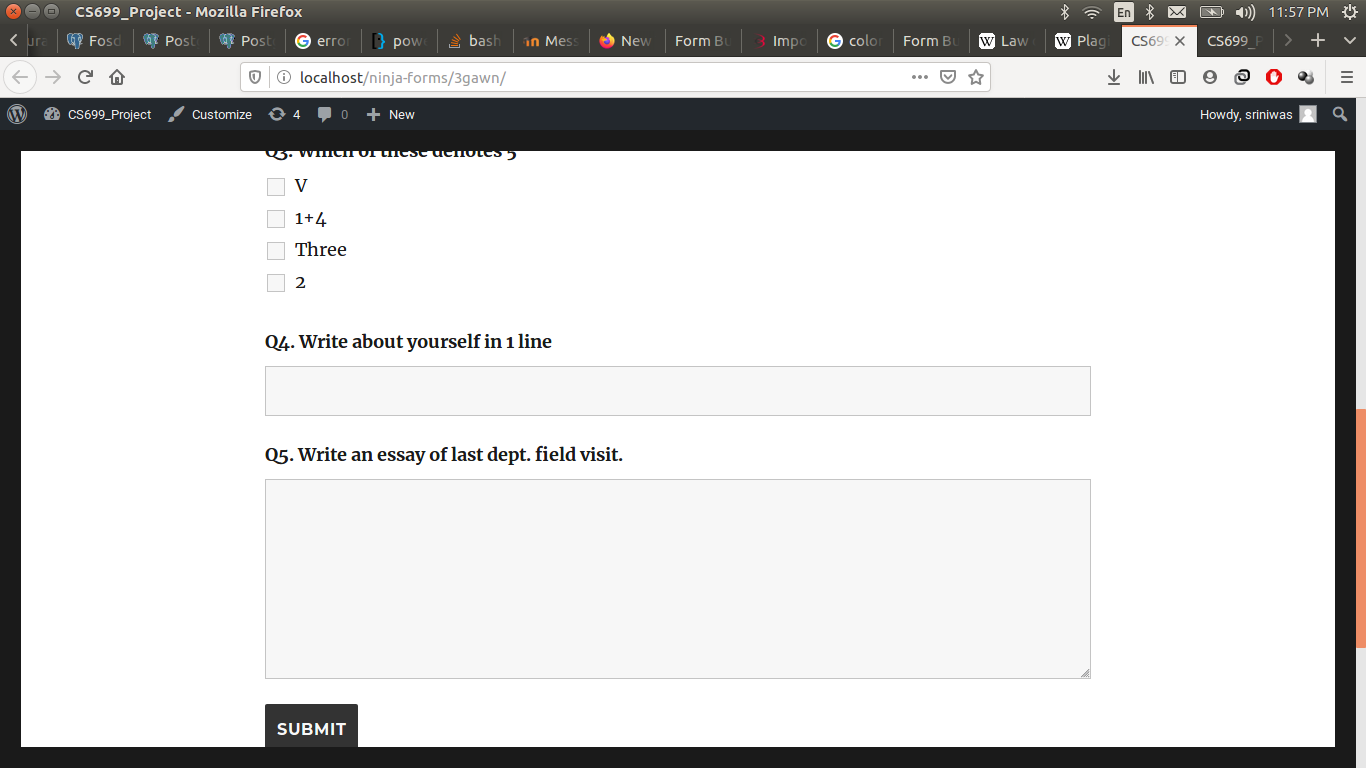
\includegraphics[width=\textwidth]{images/Test12.png}
    \caption{Demo Test1 Page 2}
  \end{minipage}
  \hfill
\end{figure} 
Every test must contain a field for roll number which will be used to detect uniquely pairwise plagiarism index among the submitted responses. Here is another example of a test.
\begin{figure}[H]
\label{fig1}
      \centering
  \begin{minipage}[b]{0.45\textwidth}
    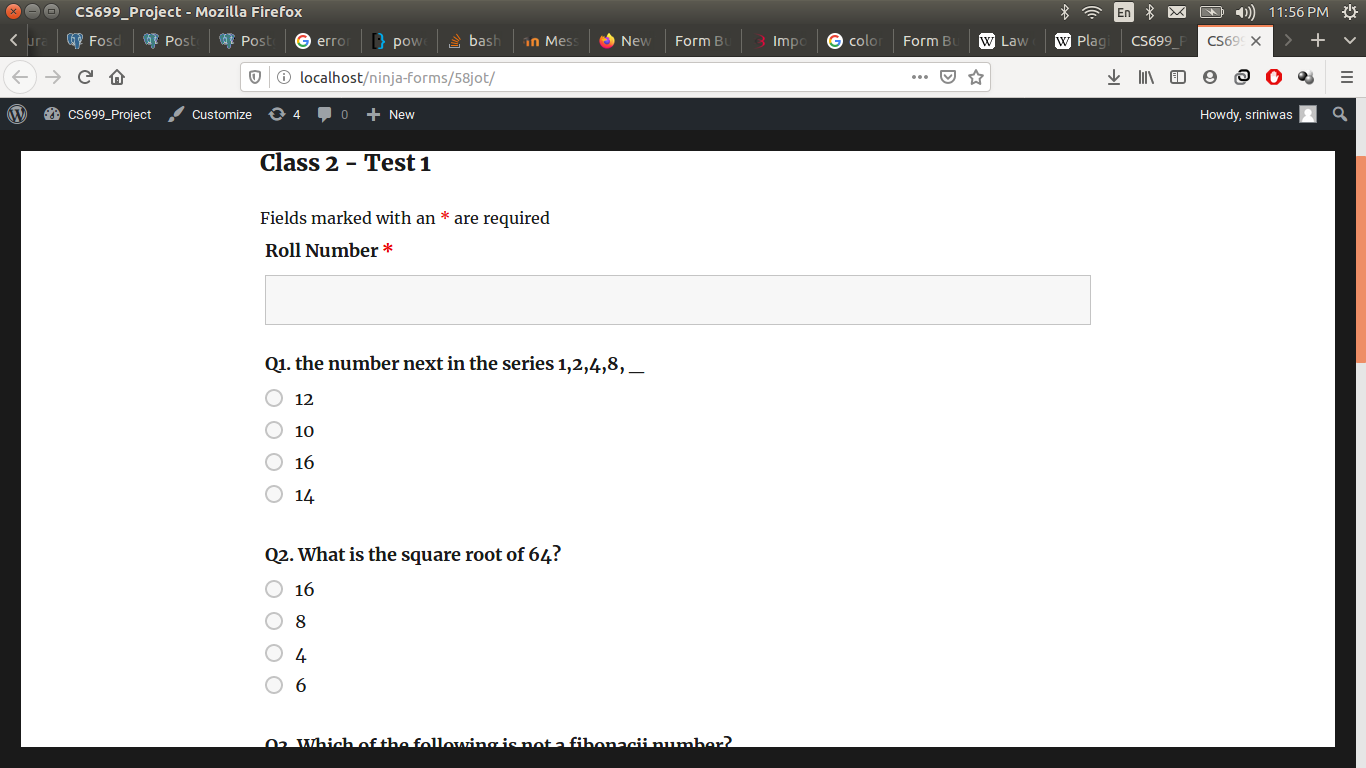
\includegraphics[width=\textwidth]{images/Test2.png}
    \caption{Demo Test2 Page 1}
  \end{minipage}
  \hfill
  \begin{minipage}[b]{0.45\textwidth}
    \includegraphics[width=\textwidth]{images/Test21.png}
    \caption{Demo Test2 Page 2}
  \end{minipage}
  \hfill
\end{figure} 
Admin can create new test using the provided interface. We are using Ninja forms plugin in wordpress for this purpose. Teacher can add any number of questions of any type in any order. And he will have to provide solutions in a csv file of the corresponding test. This is strongly required for the plagiarism detection model of ours. 
\begin{figure}[H]
    \centering
    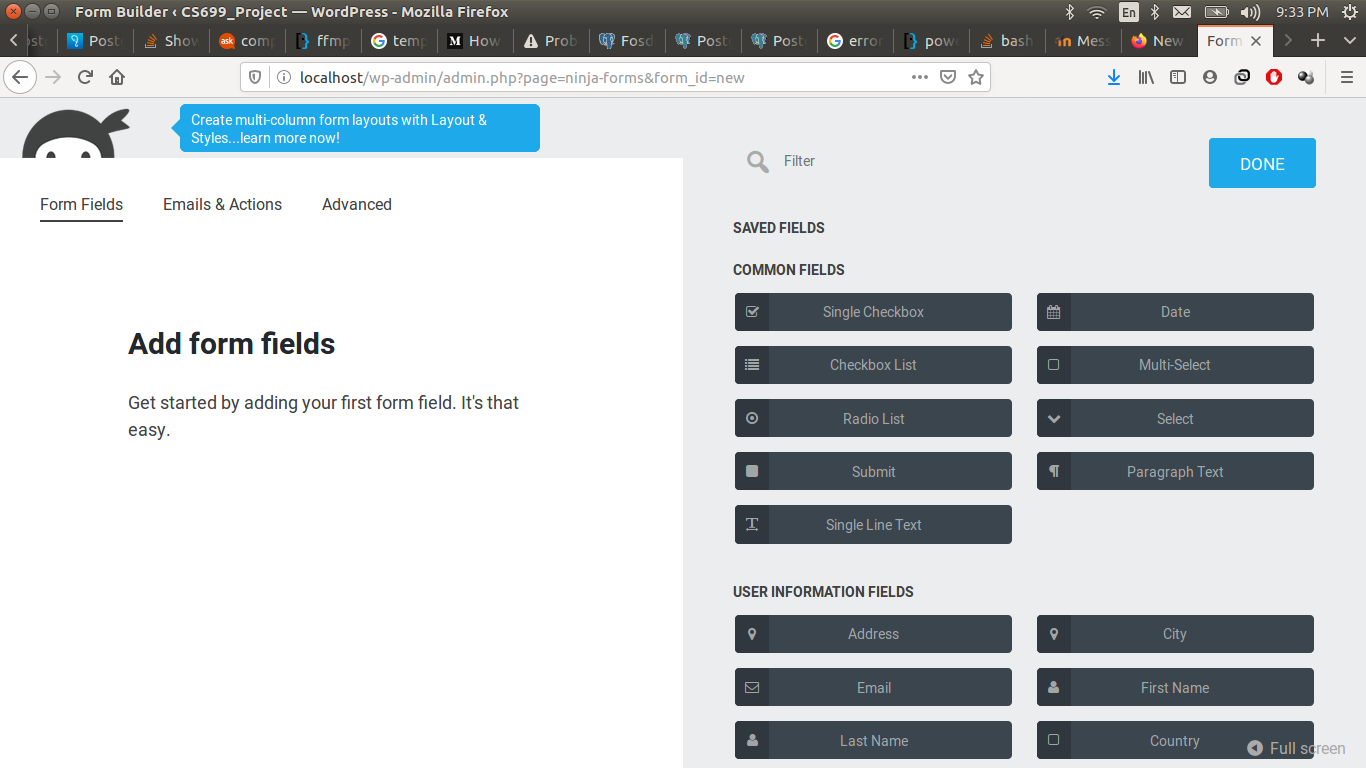
\includegraphics[width=0.5\paperwidth]{images/test_form.png}
    \caption{Sample blank form for test creation}
    \label{fig:galaxy}
\end{figure}
When deadline for attempting test is over, admin will disable the link of that test. Now after getting all the submissions/responses, while evaluating teacher will be provided with the option of applying plagiarism check or not. Also if one chooses to apply the plagiarism check while evaluating the responses, he can also customise the weights given to different algorithms according to the requirements of the test. \\
Eventually, teacher will be provided with a csv file which will have plagiarism indices in descending order for all pairs of responses. He can set a threshold passing which will mean the student has not cheated in the test.
\begin{figure}[H]
\label{fig1}
      \centering
  \begin{minipage}[b]{0.45\textwidth}
    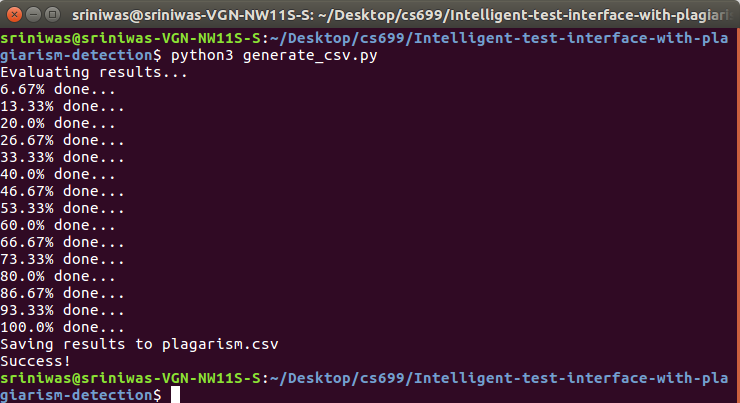
\includegraphics[width=\textwidth]{images/python_script.png}
    \caption{Running python script to evaluate plagiarism index}
  \end{minipage}
  \hfill
  \begin{minipage}[b]{0.45\textwidth}
    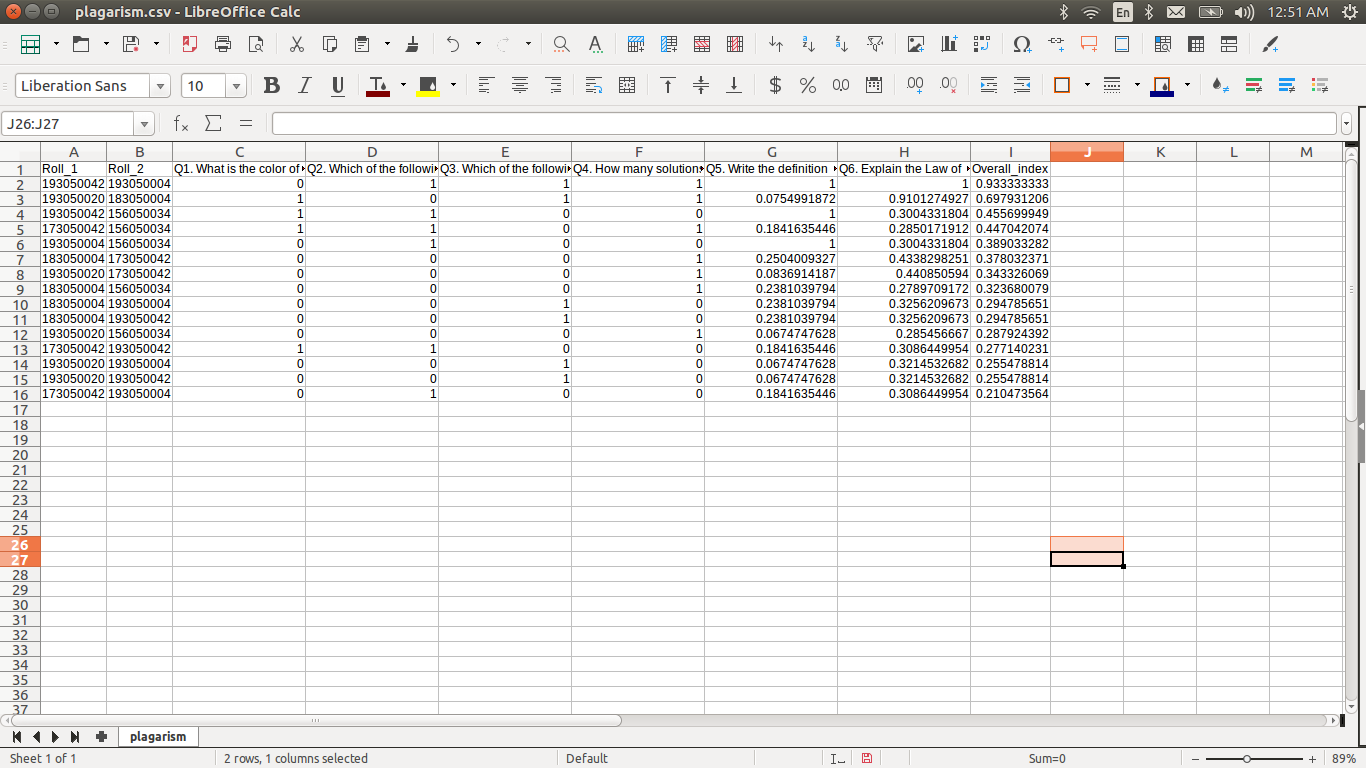
\includegraphics[width=\textwidth]{images/results_csv.png}
    \caption{CSV file consisting of plagiarism indices}
  \end{minipage}
  \hfill
\end{figure} 
If n responses are submitted in total the csv file having final result of plagiarism indices will have $\binom{N}{k}$ entries in it in sorted order(highest plagiarised index to lowest plagiarised index).

\subsection{Back End}
 A test can have briefly have two sort of questions :
 \begin{enumerate}
     \item Subjective Type (Single Line or Multiple Line)
     \item Objective Type (MCQs with single choice or multiple choice)
 \end{enumerate}
 To apply plagiarism test on subjective type questions we are using various string matching algorithms. One of the popular n-gram based similarity algorithm cosine similarity works on vectors of frequency of letters. Since results from this algorithm was significantly accurate, we modified cosine similarity for word frequency vectors and it is giving even better results. So to get best results of plagiarism indices, teacher should give this algorithm a significant weight. \\ \\
 \textbf{Weights csv file : } This file consists of weights corresponding to the algorithms Least Common Subsequence (LCS), Cosine Angle, Cosine Angle (words) and Jacard Index.
 Admin can modify these weights according to the requirements of his test. According to the weights given in this csv, the Subjective questions' plagiarism index will get evaluated. \\ \\
 \textbf{Solution csv file :} For each test teacher is supposed to provide a csv consisting of correct solutions. This csv file is useful while evaluaing the plagiarism index for MCQs. If two students have selected the same option/options then there could be two possible cases : First is that both have marked correct answer, then the chances are low that they have copied so we are giving index 0 to such a case. \\
 Second case is that both have marked same wrong option/options, here chances are comparatively high that they have copied (even higher in case of multiple choice MCQs), so we are giving index 1 to these sort of matches. Since MCQs themselves have low weightage of overall marks, in case it was just an coincidence that incorrect answers matched then also it won't effect the plagiarism index adversely until Subjective Questions of these two also caught to have some plagiarism index. \\
 
 Solution csv provided by teacher should also contain the marks distribution for the questions. After we are done evaluating individual question's plagiarism index, at the end these indices will be given weights in the ratio of their distribution of marks in the test. The outcome from this will be our final and fair Plagiarism index between those two students. 
 
 
 


\section{Technologies Used}
\subsection{Python} 
Python is a high-level, interpreted and general-purpose dynamic programming language that focuses on code readability. The syntax in Python helps the programmers to do coding in fewer steps as compared to Java or C++.The Python is widely used in bigger organizations because of its multiple programming paradigms. They usually involve imperative and object-oriented functional programming. It has a comprehensive and large standard library that has automatic memory management and dynamic features.\cite{python}\\ \\
Python has top the charts in the recent years over other programming languages like C, C++ and Java and is widely used by the programmers. The software development companies prefer Python language because of its versatile features and fewer programming codes. Nearly 14\% of the programmers use it on the operating systems like UNIX, Linux, Windows and Mac OS. The programmers of big companies use Python as it has created a mark for itself in the software development with characteristic features like-
\begin{itemize}
    \item Interactive
    \item Interpreted
    \item Modular
    \item Dynamic
    \item Object-oriented
    \item Portable
    \item High level
    \item Extensible in C++ and  C
\end{itemize}
\subsection{Wordpress}
WordPress is a simple and free Content Management System with numerous features and ample customization possibilities. It can be used to develop any kind of website, be it for a small business or for a large enterprise. \cite{word} \\ \\
Following featurs are very impressive benifits of wordpress : 
\begin{itemize}
    \item WordPress Is A Universal Platform
    \item Easy To Use
    \item Easy To Set-up
    \item  Easy To Update
    \item  Easy To Manage
    \item WordPress Is Reliable
    \item Provides Greater Accessibility
    \item Provides plugin features
\end{itemize}
\subsection{MySQL}
MySQL is a relational database management system based on SQL – Structured Query Language. The application is used for a wide range of purposes, including data warehousing, e-commerce, and logging applications. The most common use for mySQL however, is for the purpose of a web database. \cite{sql}\\
In association with a scripting language such as PHP or Perl (both offered on our hosting accounts) it is possible to create websites which will interact in real-time with a mySQL database to rapidly display categorised and searchable information to a website user.

\section{Efforts}
\subsection{Fraction of time spent in different parts of the project}

\begin{itemize}
    \item Analysis of various string matching algorithms : To get started with the project, we explored plagiarism detector software and their workings. MOSS is widely used plagiarism detector software. It is currently used by many institutes to check plagiarism over programming assignments and projects.  \\
    MOSS\cite{moss} makes it possible to objectively and automatically check all program
solutions for evidence of copying. MOSS works with programs written in C, C++, Java, Pascal, Ada and other languages and looks out for similar code structure in different documents.When someone changes the variable name or tries to introduce white spaces, some random code to deceive it, it typically does not work in their favor as the structure of the program is unchanged,while the number of token and line matches between the documents is still the same. \\
For this project we are just working on objective and subjective type of matches. We explored strsim library which implements various string similarity algorithms.
    \item Implementation of algorithm : We are using weighted combination of best performance algorithms for our task and trying to come up with an accurate and fair plagiarism index between all pairs of responses.
    \item Front and Back end development : We used wordpress for designing website for our test interface. We used Wordpress plugin Ninja for the formation of any new test.
\end{itemize}


\subsection{Fraction of work done by different team members}       
All the 3 team members contributed equally in the project with full dedication.
\section{Conclusion}
So, we have successfully created a plagiarism detecting tool for institutes/instructors. They just need to host a test and wait for the responses, and the python script will do the index calculating job. \\ \\
We have analyzed all the string matching algorithms in depth and created one for this purpose on our own too, without the help of any supporting libraries. The instructor can adjust the weights of all the algorithms in order to see the effect of various algorithms on different types of tests.\\ \\
Cosine similarity(word) metric which we created on our own showed best results for plagiarism index in large or small strings, which was a great success for our research(to come up with a modification in existing technique and get better results for a set of problems than existing techniques). \\ \\
This interface will accomplish a healthy cheat-free environment among students.
\section{Future Enhancements}
There is a wide scope of taking this project to further steps. Since plagiarism is considered as a very serious concern in institutions, Software like this which are simple but accurate are very useful. Some of the future enhancements possible in this project are as follows : 
\begin{itemize}
    \item Students can be authenticated before attempting the test.
    \item Various teachers can set tests for students
    \item There can be a course factor also there. Students enrolled to some specific course only attempt quiz or test of that course
    \item Teacher can add or remove students from his course
    \item Automatic mails can be sent to the students who crossed the threshold of plagiarism set by the test taker
    \item Android version of the same could also be a part of future enhancement
\end{itemize}

\section{References}
\makeatletter
\renewcommand{\chapter}{\@gobbletwo}
\makeatother
\begin{thebibliography}{}

\bibitem{plag} \url{https://www.thoughtco.com/plagiarism-definition-1691631}
\bibitem{wiki} \url{ https://en.wikipedia.org/wiki/Plagiarism_detection}
\bibitem{word} \url{https://wordpress.com/}
\bibitem{strsim} \url{https://pypi.org/project/strsim/}
\bibitem{moss} \url{https://theory.stanford.edu/~aiken/moss/}
\bibitem{python} \url{https://medium.com/@mindfiresolutions.usa/}
\bibitem{word} \url{https://capsicummediaworks.com/why-wordpress-is-the-best-cms/}
\bibitem{sql} \url{https://www.123-reg.co.uk/support/servers/what-is-mysql-and-why-do-i-need-it/}
\end{thebibliography}
}
\end{document}

